%% LyX 2.1.4 created this file.  For more info, see http://www.lyx.org/.
%% Do not edit unless you really know what you are doing.
\documentclass[english,nohyper]{tufte-book}
\usepackage[T1]{fontenc}
\usepackage[latin9]{inputenc}
\usepackage{units}
\usepackage{amsmath}
\usepackage{amssymb}
\usepackage{graphicx}

\makeatletter

%%%%%%%%%%%%%%%%%%%%%%%%%%%%%% LyX specific LaTeX commands.

\title{Improving the Robustness of Visual-Inertial Extended Kalman Filtering}
\author{James Jackson, Tim Mclain}

\makeatother

\usepackage{babel}
\begin{document}
\maketitle
\global\long\def\xhat{\mathbf{\hat{\mathbf{x}}}}
\global\long\def\dxhat{\hat{\dot{\mathbf{x}}}}
\global\long\def\x{\mathbf{x}}
\global\long\def\z{\mathbf{z}}
\global\long\def\i{\mathbf{i}}
\global\long\def\j{\mathbf{j}}
\global\long\def\k{\mathbf{k}}
\global\long\def\u{\mathbf{u}}
\global\long\def\norm#1{\left\Vert #1\right\Vert }
\global\long\def\skew#1{\left\lfloor #1\right\rfloor }

\section{Introduction}
\begin{itemize}
\item visual inertial navigation methods have been shown to be effective
ways to operate autonomously without GPS or other global sensors
\item features tracked through image frames can be used to constrain drift
of IMU and rate gyroscopes
\item A camera paired with an IMU can be a low-cost, effective way to navigate
without GPS
\item Recent results have shown promising results, but have been known to
have sometimes catastrophic failure modes.
\item There is a need for increased robustness in visual-inertial estimation
techniques.
\item one problem is that measurements to observed features are not typically
relative to a known origin
\item This can cause observability and consistency issues in estimation
approaches which assume that they are.
\item Recent methods have shown how to estimate features in the camera frame,
rather than an inertial frame.
\item This parameterization partitions the states cleanly into observable
and non-observable states, with global position and heading being
completely unobservable.
\item Wheeler shows how to periodically reset the position and heading states
such that they remain observable and consistent, and more sophisticated
methods are used for global uncertainty reconstruction
\item Another problem faced in visual inertial filtering includes estimating
states which are only partially observable, such as IMU biases or
depth to features.
\item Brink has shown that using a partial update can improve filter robustness
to these ``nuisance'' states while maintaining consistency.
\item Finally, many visual-inertial estimation approaches assume no knowledge
about system dynamics. For some applications, knowledge of system
dynamics can help improve estimation accuracy and constrain divergence
in some modes (a multirotor is unlikely to be flying at a million
miles per hour, therefore depth to features is unlikely to run to
infinity)
\item Leishman has shown a method for incorporating a linear drag model
into multirotor dynamics, which dramatically improves the estimation
accuracy and robustness.
\item In this work, we incorporate a relative reset and partial update to
a robocentric visual-inertial kalman filtering approach. 
\item We will first discuss the derivation of the filter including a new
keyframe reset step and inline partial update formulation.
\item Then, we will demonstrate this filter on a hardware dataset of a MAV
flying in a motion capture room and compare results with and without
the use of a multirotor drag dynamic approximation.
\end{itemize}

\section{Notation}

We will use the following notation

\[
\begin{aligned}q_{I}^{b} & \quad\textrm{Quaternion describing rotation from the inertial frame to the body frame}\\
v_{b/I}^{b} & \quad\textrm{velocity of the body frame, with respect to the inertial frame, expressed in the body frame}\\
p_{b/I}^{I} & \quad\textrm{position of the body, with respect to the inertial frame, expressed in the inertial frame}\\
\zeta_{i/c}^{c} & \quad\mbox{unit vector directed at feature \ensuremath{i} from the camera origin, expressed in the camera frame}\\
q_{c}^{\zeta_{i}} & \quad\mbox{quaternion which describes the rotation from the camera z axis to the unit vector \ensuremath{\zeta_{i/c}^{c}}}\\
\i,\j,\k & \quad\mbox{the orthogonal unit vectors describing the standard \ensuremath{x,y,z,}basis for a coordinate frame}
\end{aligned}
\]


We will also make extensive use of the skew-symmetric matrix, defined
as

\[
\left\lfloor v\right\rfloor =\left[\begin{array}{ccc}
0 & -v_{3} & v_{2}\\
v_{3} & 0 & -v_{1}\\
-v_{2} & v_{1} & 0
\end{array}\right]
\]


and is related to the cross-product between two vectors, that is
\[
v\times w=\left\lfloor v\right\rfloor w
\]



\subsection{Quaternions}

We will use standard Hamiltonian Notation for quaternions:

\begin{equation}
q=q_{w}+q_{x}\i+q_{y}\j+q_{z}\k=\begin{bmatrix}q_{w} & \bar{q}^{\top}\end{bmatrix}^{\top},
\end{equation}


where quaternion multiplication is defined as

\begin{equation}
p\otimes q=\begin{bmatrix}p_{w} & -\bar{p}^{\top}\\
\bar{p} & p_{w}I+\left\lfloor \bar{p}\right\rfloor 
\end{bmatrix}\begin{bmatrix}q_{w}\\
\bar{q}
\end{bmatrix}.
\end{equation}


The $3\times3$ rotation matrix based on a quaternion is defined as

\begin{equation}
R\left(q\right)=\left(2q_{w}^{2}-1\right)I-2q_{w}\left\lfloor \bar{q}\right\rfloor +2\bar{q}\bar{q}^{\top}\in\mathbb{R}^{3\times3},
\end{equation}


and is defined as a passive rotation. That is, $R\left(q_{i}^{b}\right)r$
results in the original vector $r$ expressed in the new coordinate
frame $i$. The transpose of the rotation matrix results in an active
rotation, where $R\left(q_{i}^{b}\right)^{\top}r$ results in a new
rotated version of vector $r$, expressed in the original frame.

The exponential mapping for a quaternion is defined as 

\begin{equation}
\exp\left(\delta\right)=\begin{bmatrix}q_{w}\\
\bar{q}
\end{bmatrix}=\begin{bmatrix}\cos\left(\frac{\lVert\delta\rVert}{2}\right)\\
\sin\left(\frac{\lVert\delta\rVert}{2}\right)\frac{\delta}{\lVert\delta\rVert}
\end{bmatrix},
\end{equation}


\begin{equation}
\log\left(q\right)=2\mathrm{atan2}\left(\left\Vert \bar{q}\right\Vert ,q_{w}\right)\frac{\bar{q}}{\left\Vert \bar{q}\right\Vert },
\end{equation}


with the small-angle approximations (when $\norm{\delta}<10^{-4}$)

\begin{eqnarray*}
\exp\left(\delta\right) & \approx & \left[\begin{array}{c}
1\\
\frac{\delta}{2}
\end{array}\right]\\
\log\left(q\right) & \approx & 2\textrm{sign}\left(q_{w}\right)\bar{q}
\end{eqnarray*}



\subsection{$\boxplus$ and $\boxminus$ operators}

\cite{key-1}Introduces a new syntax to simplify working with the
manifold representation of Lie Groups and introduced the $\boxplus$
and $\boxminus$ operators. We will use this syntax. One common application
of this syntax can be seen below in the descretized quaternion dynamics
(where $\theta=\omega dt$)

\begin{eqnarray}
q_{t+1} & = & q_{t}\boxplus\theta\\
\theta & = & q_{1}\boxminus q_{2}.
\end{eqnarray}


It is important to note that the dimensionalities of $\omega$ and
$q$ are different. The $\boxplus$ and $\boxminus$ operators are
defined for quaternions as follows:

\begin{eqnarray}
\boxplus: & SO\left(3\right)\times\mathbb{R}^{3} & \rightarrow SO\left(3\right),\nonumber \\
 & q,\theta & \mapsto q\otimes\exp\left(\theta\right),\\
\boxminus: & SO\left(3\right)\times SO\left(3\right) & \rightarrow\mathbb{R}^{3},\nonumber \\
 & q,p & \log\left(p\otimes q^{-1}\right).
\end{eqnarray}


This new syntax allows us to work with these parameterizations as
if they were vectors. These operators become the equivalent of vector
addition and subtraction, and therefore allow proper defintions of
derivatives and integrals across these operators. A properly defined
$\boxplus$ manifold must obey the following identies:

\begin{eqnarray}
 & x\boxplus0 & =x\\
\forall y\in S:\quad & x\boxplus\left(y\boxminus x\right) & =y\\
\forall\delta\in V:\quad & (x\boxplus\delta)\boxminus x & =\delta\\
\forall\delta_{1}\delta_{1}\in\mathbb{R}^{n}:\quad & \lVert(x\boxplus\delta_{1})\boxminus(x\boxplus\delta_{2})\rVert & \leq\lVert\delta_{1}-\delta_{2}\rVert
\end{eqnarray}


These operators must also form a diffeomorphism from $V$ to $S$,
so that derivatives of $\delta$ correspond to limits of $x\boxplus\delta$.
For example, the derivative of a quaternion, as defined using the
$\boxplus$ and $\boxminus$ operators are

\begin{eqnarray}
\dfrac{\partial}{\partial x}q(x) & : & =\lim_{\epsilon\rightarrow0}\dfrac{q(x+\epsilon)\boxminus q(x)}{\epsilon}\\
\dfrac{\partial}{\partial q}x(q) & : & =\lim_{\epsilon\rightarrow0}\left[\begin{array}{c}
\dfrac{x\left(q\boxplus(\mathbf{i}\epsilon)\right)-x\left(q\right)}{\epsilon}\\
\dfrac{x\left(q\boxplus(\mathbf{j}\epsilon)\right)-x\left(q\right)}{\epsilon}\\
\dfrac{x\left(q\boxplus(\mathbf{k}\epsilon)\right)-x\left(q\right)}{\epsilon}
\end{array}\right]^{\top}
\end{eqnarray}


Derivatives over all $\boxplus$ and $\boxminus$ operators can be
found in a similar manner. This allows us to use this operator to
define dynamics and Jacobians across our non-linear manifold representations.

We can represent covariance using the $\boxplus$ and $\boxminus$
operators in the following method

\begin{equation}
\mathcal{N}\left(\mu,\Sigma\right):=\mu\boxplus\mathcal{N}\left(0,\Sigma\right)
\end{equation}


It is important to note here that in many cases,
\begin{align}
\mu\in\mathbb{R}^{m}\\
\Sigma\in\mathbb{R}^{n\times n}\\
m\neq n
\end{align}



\subsection{Feature Bearing Parameterization}

As in Bloesch, we parameterize the bearing states to features in the
camera frame as rotations in $SE\left(3\right)$ which describe the
rotation from the camera z-axis to the bearing vector directed at
the feature. Let $\zeta_{i/c}^{c}$ be the 3D unit vector directed
at feature $i$, with respect to the camera frame $c$. We then define
$q_{c}^{\zeta_{i}}$as the quaternion rotation between $\mathbf{k}$,
the z-axis of the camera frame and the 3D unit bearing vector$\zeta_{i/c}^{c}$.
The change between two 3D unit vectors $\zeta_{i}$ and $\zeta_{j}$
can be described using an axis-angle representation, where the direction
of the axis of rotation is perpendicular to both of the 3D unit vectors,
scaled by the angle. This is shown in the figure below.

\begin{figure}
\begin{centering}
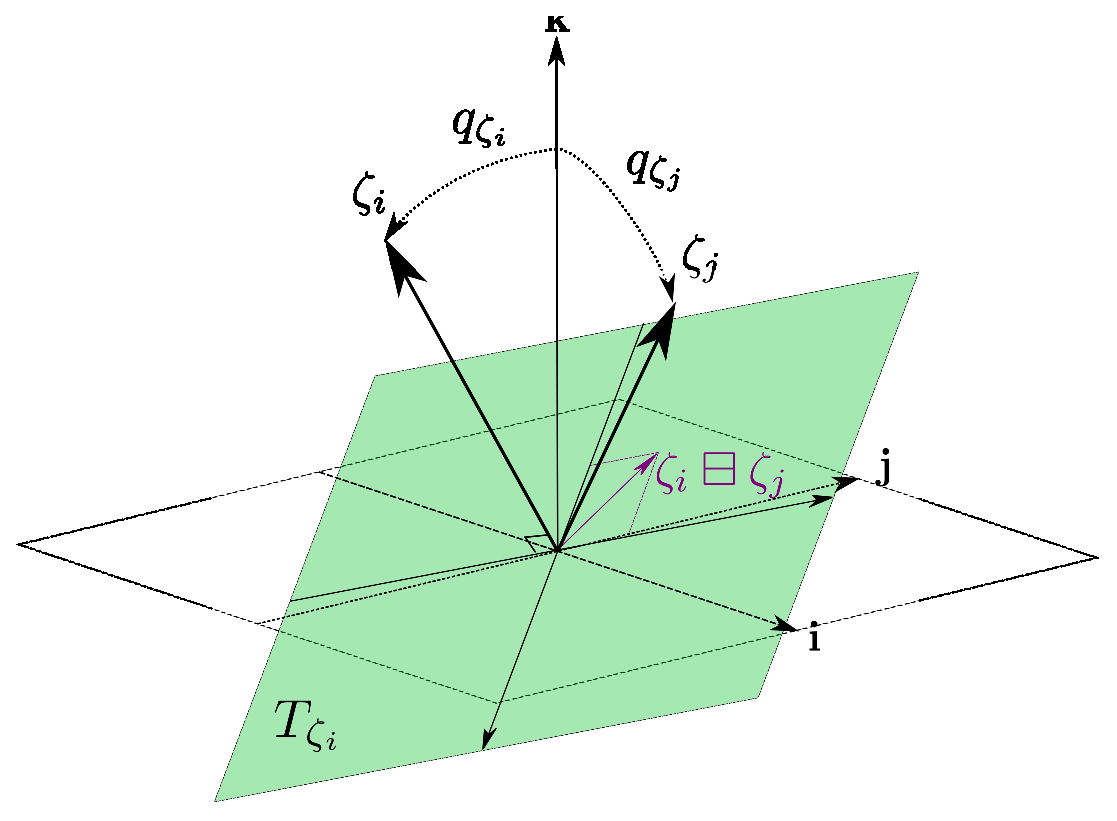
\includegraphics[width=0.8\columnwidth]{/home/superjax/dev_ws/src/vi_ekf/latex/figures/feature_diagram}
\par\end{centering}

\caption{Illustration of Bearing Vector Geometry}
\end{figure}


As can be seen in the picture, there are only 2 degrees of freedom
in this parameterization because the axis of rotation is always in
the plane normal to $\zeta_{i}$. Therefore, we can define a projection
matrix $T_{\zeta_{i}}$, which reduces the dimensionality of the axis-angle
representation to this plane. It is important to note the active rotation
being applied in both cases. 

\begin{eqnarray}
\zeta_{i/c}^{c} & = & R\left(q_{c}^{\zeta_{i}}\right)^{\top}\k\in\mathcal{S}^{2}\subset\mathbb{R}^{3}\\
T_{\zeta_{i}} & = & R\left(q_{c}^{\zeta_{i}}\right)^{\top}\left[\begin{array}{cc}
\i & \j\end{array}\right]\in\mathbb{R}^{3\times2}
\end{eqnarray}


Here are the definitions of the $\boxplus$ and $\boxminus$ operators
of this space

\begin{eqnarray}
\boxplus: & SO\left(3\right)\times\mathbb{R}^{2} & \rightarrow SO\left(3\right),\nonumber \\
 & q_{\zeta},\delta & \mapsto\exp(T_{\zeta}\delta)\otimes q_{\zeta},\\
\boxminus: & SO\left(3\right)\times SO\left(3\right) & \rightarrow\mathbb{R}^{2},\nonumber \\
 & q,p & \mapsto\theta T_{\zeta_{j}}^{\top}s\left(q_{\zeta_{i}},q_{\zeta_{j}}\right),
\end{eqnarray}
where $\theta$ is the angle between the two unit bearing vectors
$\zeta_{i}$ and $\zeta_{j}$
\[
\theta=\cos^{-1}\left(\zeta_{i}^{\top}\zeta_{j}\right),
\]
and 

\[
s\left(q_{\zeta_{i}},q_{\zeta_{j}}\right)=\dfrac{\zeta_{j}\times\zeta_{i}}{\lVert\zeta_{j}\times\zeta_{i}\rVert}
\]
is the axis of rotation between the bearing vectors.

With only two degrees of freedom, and with all feature vectors referencing
the camera $z$ axis, there are an infinite number of quaternions
which can be used to represent the same unit vector. The difference
between these rotations is some angle of rotation about the bearing
vector $\zeta$ itself, which is removed by the projection operation
and can therefore be neglected.


\section{Derivation}

Here we will derive the relevant geometry and dynamics to fully describe
and implement our version of the filter. First, we will briefly present
some identities that will be helpful in later derivations.

Some helpful identities when dealing with skew-symmetric and rotation
matrices

\[
\skew vw=-\skew wv
\]


\begin{equation}
\left\lfloor Rv\right\rfloor =R\left\lfloor v\right\rfloor R^{\top}\label{eq:skew_rotation}
\end{equation}


The time derivative of a rotation matrix between two arbitrary (possibly
time varying) frames is

\[
\begin{aligned}\frac{d}{dt}R\left(q_{a\left(t\right)}^{b\left(t\right)}\right) & =\left\lfloor \omega_{b\left(t\right)/a\left(t\right)}^{b\left(t\right)}\right\rfloor R\left(q_{a\left(t\right)}^{b\left(t\right)}\right)\end{aligned}
,
\]
however, if the rotation matrix is with respect to a fixed frame,
this can be simplified

\[
\begin{aligned}\frac{d}{dt}R\left(q_{a}^{b\left(t\right)}\right) & =\left\lfloor \omega_{b\left(t\right)/a}^{b\left(t\right)}\right\rfloor R\left(q_{a}^{b\left(t\right)}\right).\end{aligned}
\]
On the other hand, if the rotation matrix is defined with respect
to a time-varying frame and describes the rotation to a fixed frame,
(such as in the case of body-fixed dynamics) we can perform some manipulation
using \ref{eq:skew_rotation} to put the result into a more convenient
frame

\begin{eqnarray}
\frac{d}{dt}R\left(q_{b\left(t\right)}^{a}\right) & = & \left\lfloor \omega_{a/b\left(t\right)}^{a}\right\rfloor R\left(q_{b\left(t\right)}^{a}\right)\nonumber \\
 & = & \left\lfloor R\left(q_{b\left(t\right)}^{a}\right)\omega_{a/b\left(t\right)}^{b\left(t\right)}\right\rfloor R\left(q_{b\left(t\right)}^{a}\right)\nonumber \\
 & = & R\left(q_{b\left(t\right)}^{a}\right)\left\lfloor \omega_{a/b\left(t\right)}^{b\left(t\right)}\right\rfloor R\left(q_{a}^{b\left(t\right)}\right)R\left(q_{b\left(t\right)}^{a}\right)\nonumber \\
 & = & R\left(q_{b\left(t\right)}^{a}\right)\left\lfloor \omega_{a/b\left(t\right)}^{b\left(t\right)}\right\rfloor \nonumber \\
 & = & -R\left(q_{b\left(t\right)}^{a}\right)\left\lfloor \omega_{b\left(t\right)/a}^{b\left(t\right)}\right\rfloor .\label{eq:body_fixed_rotation_dynamics}
\end{eqnarray}


The derivative of a passively rotated vector, with respect to the
quaternion describing the rotation is

\[
\begin{aligned}\frac{d}{dq_{a}^{b}}\left(R\left(q_{a}^{b}\right)v\right) & =-\left\lfloor R\left(q_{a}^{b}\right)v\right\rfloor ,\end{aligned}
\]
while the derivative of an actively rotated vector to the same is

\[
\begin{aligned}\frac{d}{dq_{a}^{b}}\left(R\left(q_{a}^{b}\right)^{\top}v\right) & =-\left\lfloor R\left(q_{a}^{b}\right)^{\top}v\right\rfloor \\
 & =-R\left(q_{a}^{b}\right)^{\top}\left\lfloor v\right\rfloor R\left(q_{a}^{b}\right).
\end{aligned}
\]


The derivative of the projection operator with respect to the feature
quaternion to the unit vector is

\[
\begin{aligned}\frac{d}{dq_{c}^{\zeta}}\left(T_{\zeta}^{\top}v\right) & =\frac{d}{dq_{c}^{\zeta}}\left(\left[\begin{array}{cc}
\i & \j\end{array}\right]^{\top}R\left(q_{c}^{\zeta}\right)v\right)\\
 & =-\left[\begin{array}{cc}
\i & \j\end{array}\right]^{\top}\left\lfloor R\left(q_{c}^{\zeta}\right)v\right\rfloor \left[\begin{array}{cc}
\i & \j\end{array}\right]\\
 & =-\left[\begin{array}{cc}
\i & \j\end{array}\right]^{\top}R\left(q_{c}^{\zeta}\right)\left\lfloor v\right\rfloor R\left(q_{c}^{\zeta}\right)^{\top}\left[\begin{array}{cc}
\i & \j\end{array}\right]\\
 & =-T_{\zeta}^{\top}\left\lfloor v\right\rfloor T_{\zeta},
\end{aligned}
\]
and the derivative of a bearing vector with respect to the quaternion
is

\[
\begin{aligned}\frac{d}{dq_{\zeta}^{c}}\zeta^{c} & =\frac{d}{dq_{\zeta}^{c}}\left(R\left(q_{\zeta}^{c}\right)^{\top}\k\right)\\
 & =\left\lfloor \zeta\right\rfloor T_{\zeta}.
\end{aligned}
\]



\subsection{State Definition}

The state vector in our implementation is defined as follows with
$\rho_{i}$ as the inverse depth to feature $i$:

\[
\boldsymbol{x}=\left[p_{b/I}^{I},v_{b/I}^{b},q_{I}^{b},\beta_{a},\beta_{\omega},\mu,q_{c}^{\zeta_{0}},\rho_{0}\cdots q_{c}^{\zeta_{n}},\rho_{n}\right]^{\top}\in\mathbb{R}^{17+5n}.
\]


The covariance matrix $P$ is defined as 
\[
P=E\left[\hat{\boldsymbol{x}}\boxminus\boldsymbol{x}\right]E\left[\hat{\boldsymbol{x}}\boxminus\boldsymbol{x}\right]^{\top}\in\mathbb{R}^{\left(16+3n\right)\times\left(16+3n\right)}.
\]



\subsection{State Dynamics}

Below are the dynamics of a multirotor using a linearized drag term
with $\beta_{a}$and $\beta_{\omega}$ as the accelerometer and gyro
constant biases, and $\mu$ as a constant linear drag term. For the
derivation of the linear drag term, we refer to Leishman

\begin{eqnarray}
\dot{p}_{bI}^{I} & = & R^{\top}\left(q_{I}^{b}\right)v_{b/I}^{b}\nonumber \\
\dot{v}_{b/I}^{b} & = & \left\lfloor v_{b/I}^{b}\right\rfloor \boldsymbol{\omega}_{b/I}^{b}+R\left(q_{I}^{b}\right)g+\k\k^{\top}\left(y_{a}-\beta_{a}\right)-\mu_{t}\left[\begin{array}{ccc}
\i & \j & 0\end{array}\right]v_{b/I}^{b}+\eta_{v}\label{eq:velocity_dynamics}\\
\dot{q}_{I}^{b} & = & \omega\nonumber \\
\dot{\beta}_{a} & = & \eta_{\beta_{a}}\nonumber \\
\dot{\beta}_{\omega} & = & \eta_{\beta_{\boldsymbol{\omega}}}\nonumber \\
\dot{\mu} & = & \eta_{\mu}d\nonumber 
\end{eqnarray}


For the derivation of the feature bearing and inverse depth dynamics,
we refer the reader to Appendix A.

\begin{eqnarray*}
\dot{q}_{c}^{\zeta} & = & T_{\zeta}^{\top}\left(\omega_{c/I}^{c}-\rho_{i}\left\lfloor \zeta_{i}^{c}\right\rfloor v_{c/I}^{c}\right)\\
\dot{\rho} & = & \rho^{2}\zeta_{i}^{c}{}^{\top}v_{c/I}^{c}
\end{eqnarray*}



\subsection{Continuous-Discrete EKF Equations}

We will use the following formulation of the continuous-discrete EKF
equations on the manifold with state $\xhat$ and input $\u$ and
$\dot{\x}=f\left(\x,\u\right)$

\[
\begin{aligned}\xhat\left(t+dt\right) & =\xhat\left(t\right)\boxplus f\left(\xhat\left(t\right),\mathbf{\u}\left(t\right)\right)dt\\
A & =\left.\frac{\partial f}{\partial\x}\right|_{\x=\xhat\left(t\right)}\\
G & =\left.\frac{\partial f}{\partial\u}\right|_{\x=\xhat\left(t\right)}\\
P\left(t+dt\right) & =P\left(t\right)+\left(AP\left(t\right)+P\left(t\right)A^{\top}+GQ_{\u}G+Q_{\x}\right)dt
\end{aligned}
\]
and the following measurement update equations for a generic measurement
$\mathbf{z}_{y}=h_{y}\left(\mathbf{x}\right)$

\[
\begin{aligned}H_{y} & =\frac{\partial h_{y}}{\partial\x}\\
K & =PH_{y}^{\top}\left(R_{y}+H_{y}PH_{y}^{\top}\right)^{-1}\\
P^{+} & =(I-KH_{y})P^{-}\\
\hat{\x}^{+} & =\hat{\x}\boxplus K\left(\mathbf{z}_{y}\boxminus h_{y}\left(\hat{\x}\right)\right)
\end{aligned}
\]


For derivation of the Jacobians $\frac{\partial f}{\partial\x}$ and
$\frac{\partial f}{\partial\u}$, we refer the reader to Appendix
B.


\subsection{Measurement Models}

To reduce modeling errors, we incorporate pixel measurements directly
into our filter using the following model. Let us consider a pixel
measurement $\lambda$ given focal length $f$ and feature bearing
vector $\zeta$, and using the geometry showing in Figure\ref{fig:pixel_geometry},
and solve for the distance along the bearing vector to the image plane
$s$, we get

\[
\begin{aligned}\k^{\top}\left(-f\k+s\zeta\right) & =0\\
\left(\k^{\top}s\zeta\right)-f\left(\k^{\top}\k\right) & =0\\
s\left(\k^{\top}\zeta\right) & =f\left(\k^{\top}\k\right)\\
s & =\frac{f}{e_{z}\zeta}.
\end{aligned}
\]


If we use this scaling factor to map into pixel coordinates, (where
$\left(0,0\right)$ is located at the top of the image, with center
pixel $\lambda_{c}=\left[c_{x},c_{y}\right]^{\top}$ and split $f$
into focal lengths $f_{x}$ and $f_{y}$) we get the following expression
for pixel locations given a particular feature bearing vector $\zeta$.

\begin{eqnarray}
h_{\lambda_{i}}(x,u,\eta_{\lambda_{i}}) & = & \left[\begin{array}{ccc}
1 & 0 & 0\\
0 & 1 & 0
\end{array}\right]s\zeta_{i}+\lambda_{c}+\eta_{\lambda_{i}}\nonumber \\
 & = & \left[\begin{array}{ccc}
f_{x} & 0 & 0\\
0 & f_{y} & 0
\end{array}\right]\frac{1}{\k\zeta_{i}}\zeta_{i}+\lambda_{c}+\eta_{\lambda_{i}}\nonumber \\
 & = & F\frac{1}{\k\zeta_{i}}\zeta_{i}+\lambda_{c}+\eta_{\lambda_{i}}.\label{eq:pixel_meas_model}
\end{eqnarray}


This model is inherently very non-linear with respect to the bearing
vector. Therefore characterizing noise as normal about the pixel measurement
then mapping into the bearing vector space will improve uncertainty
consistency when compared to characterizing noise about the bearing
vector itself.

\begin{figure}[h]
\begin{centering}
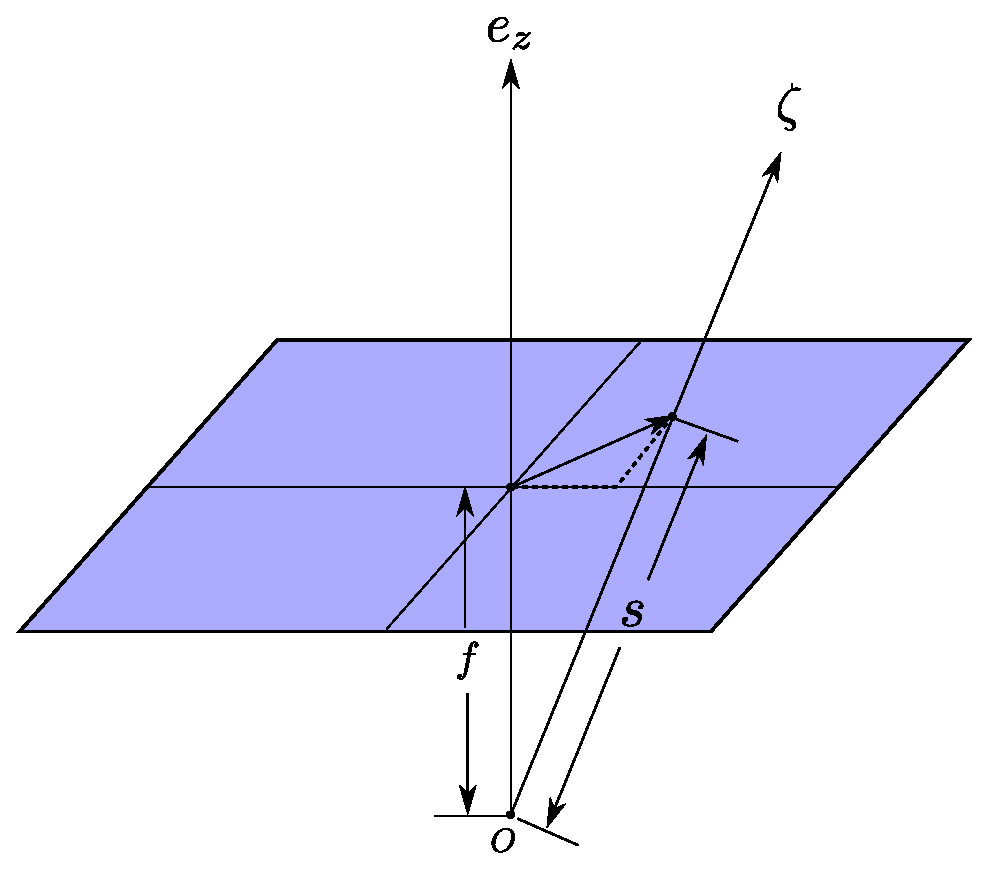
\includegraphics[width=0.8\textwidth]{/home/superjax/dev_ws/src/vi_ekf/latex/figures/pixel_geometry}
\par\end{centering}

\begin{centering}
\label{fig:pixel_geometry}
\par\end{centering}

\caption{Camera Pixel and feature vector geometry}
\end{figure}


Using the multirotor drag model in \ref{eq:velocity_dynamics} provides
the benefit that velocity becomes directly observed by the accelerometer
(assuming a linear drag constant). To derive this fact, we start with
the sum of the forces acting on the multirotor body. These are assumed
to be gravity ($mg$), thrust ($T$) and drag ($\mu mv$)

\begin{eqnarray*}
ma_{b/I}^{b} & = & \sum F^{b}\\
 & = & R\left(q_{I}^{b}\right)mg-\mu mv_{b/i}^{b}+T\\
a_{b/I}^{b} & = & R\left(q_{I}^{b}\right)g-\mu v_{b/i}^{b}+\frac{T}{m}
\end{eqnarray*}
The accelerometer measures all applied accelerations, except gravity,
with the addition of the constant bias term $\beta_{a}$ and noise
$\eta_{a}$

\begin{eqnarray}
\z_{y} & = & a_{b/I}^{b}-R\left(q_{I}^{b}\right)g+\beta_{a}+\eta_{a}\nonumber \\
 & = & R\left(q_{I}^{b}\right)g-\mu v_{b/i}^{b}+\frac{T}{m}-R\left(q_{I}^{b}\right)g+\beta_{a}+\eta_{a}\nonumber \\
 & = & \frac{T}{m}-\mu v_{b/i}^{b}+\beta_{a}+\eta_{a}\label{eq:accel_xyz}
\end{eqnarray}


If we assume that $T$ acts only along the $\k$ axis, then we can
remove its influence by considering only the $x$ and $y$ axes of
\ref{eq:accel_xyz}

\begin{equation}
h_{acc}\left(x,u,\eta_{a}\right)=I_{2\times3}\left(\frac{T}{m}-\mu v_{b/i}^{b}+\beta_{a}+\eta_{a}\right)\label{eq:accel_model}
\end{equation}


The associated Jacobians of \ref{eq:pixel_meas_model} and \ref{eq:accel_model}
are given in Appendix C with the addition of several other, simpler
measurement models used in this work.


\subsection{Keyframe Reset}

As shown in Wheeler and Koch, performing a ``Keyframe Reset'' when
global states are unobservable can dramatically improve filter consistency
and accuracy. A keyframe reset is performed by resetting the global
position and heading states to zero, and updating the covariances
appropriately. Each reset step results in a new ``node'' being declared
in a pose graph-like structure in $SE\left(2\right)$ which can be
optimized using higher-order methods to properly incorporate loop
closures and other measurements. See Figure \ref{fig:keyframe_geometry}
for an illustration of the coordinate frames involved in the keyframe
reset.

\begin{figure}[h]
\begin{centering}
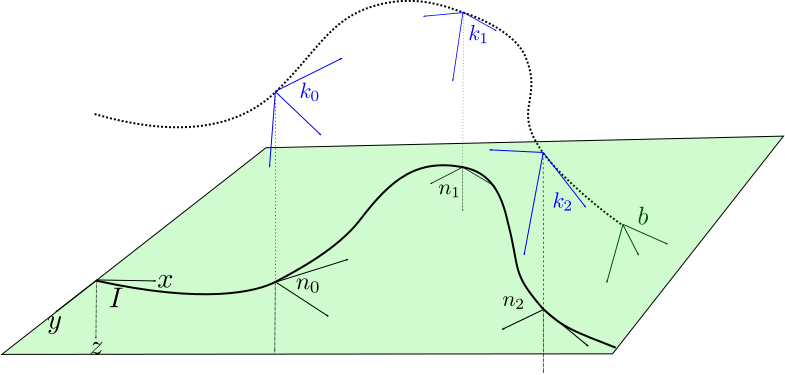
\includegraphics[width=0.8\textwidth]{figures/keyframes}
\par\end{centering}

\begin{centering}
\label{fig:keyframe_geometry}
\par\end{centering}

\caption{Keyframe Coordinate Frames}
\end{figure}


While resetting the position states is trivial, resetting rotation
about $\k$ in the attitude quaternion $q_{I}^{b}$ is more complicated.
In Koch, this reset step was derived using an intermediate euler-angle
decomposition. In this work, we directly update the quaternion, without
euler angle calculations and using manifold operations. 

Consider a quaternion $q^{-}$ and unit vector$u$. We wish to remove
all rotation in $q^{-}$ about $u$ and extract a new quaternion $q^{+}$.
We can do this by rotating $u$ by $q^{-}$, which results in a new
vector $v$. Because the shortest rotation between these two vectors
would have no component of rotation about either $u$ or $v$, we
can extract $q^{+}$ using the exponential map on an axis-angle parameterization
of the difference.

\begin{eqnarray*}
v & = & R\left(q^{-}\right)^{\top}u\\
\theta & = & u^{\top}v\\
s & = & \left\lfloor u\right\rfloor v\\
q^{+} & = & \exp\left(\theta s\right)
\end{eqnarray*}


Using this fact, the actual reset can performed in the manner described
in Koch: 

\[
p_{b/n}^{n,+}=\left[\begin{array}{c}
0\\
0\\
\k^{\top}p_{b/n}^{n,-}
\end{array}\right]
\]


\[
q_{n}^{b,+}=\exp\left(\k\left(R\left(q_{n}^{b,-}\right)^{\top}\k\right)\left(\skew{\k}R\left(q_{n}^{b,-}\right)^{\top}\k\right)\right)
\]


\[
P^{+}=NPN^{\top},
\]


where $N$ is given in Appendix D. No reset step is required for feature
states, as they are defined with respect to the camera frame directly
and are therefore not subject to the same observability problems as
global position and heading. If feature states are defined in an inertial
frame, which is the case for many visual-inertial filtering methods,
a keyframe reset is not straight-forward. 


\subsection{Partial Update}

\global\long\def\blambda{\mathbf{\boldsymbol{\lambda}}}


A common difficulty faced in visual-inertial navigation is the estimation
of ``nuisance'' states which may only be partially observable during
many maneuvers. In this filter, these states include the inverse depth
to each feature, $\rho_{i}$, accel and gyro biases $\beta_{a}$ and
$\beta_{\omega}$, and the linear drag term $\mu$. As noted by Brink,
estimating these terms in the traditional manner can cause filter
divergence, but ignoring them or considering them as known constants
would produce an overconfident estimate. Therefore, because of the
abundance of these states in our system, we employ a version of the
Partial-Update Schmidt-Kalman Filter as proposed by Brink. This method
allows the designer to ``dial'' the effect of a measurement update
on a particular state, with a scalar gain $\gamma_{i}$. While this
method loses any guarantees about optimality in estimating these states
in a kalman filtering framework, In Brink it was shown to speed up
convergence of these nuisance states by limiting the effect of linearization
errors when applied to the non-linear IMU-camera estimation problem.
If we properly map the uncertainty through this partial update, our
extended kalman filter can remain consistent and not be subject to
as severe linearization errors. 

In Brink, we are presented with the following form of the update step:

\begin{eqnarray*}
\xhat^{+} & = & \xhat^{-}+K\left(\z-H\xhat^{-}\right)\\
P^{+} & = & \left(I-KH\right)P^{-}\\
\cdots & \cdots & \cdots\\
\hat{x}_{i}^{++} & = & \gamma_{i}\hat{x}_{i}^{-}+\left(1-\gamma_{i}\right)\hat{x}_{i}^{+}\\
P_{ij}^{++} & = & \gamma_{i}\gamma_{j}P_{ij}^{-}+\left(1-\gamma_{i}\gamma_{j}\right)P_{ij}^{-}.
\end{eqnarray*}
The drawback of this formulation is the intermediate calculation of
$\xhat^{+}$and $P^{+}$. We can manipulate these equations to remove
this intermediate calculation, but maintain algebraic equivalence.
Let us first define $\lambda_{i}=1-\gamma_{i}$

\begin{eqnarray*}
\hat{x}_{i}^{++} & = & \left(1-\lambda_{i}\right)\hat{x}^{-}+\lambda_{i}\hat{x}_{i}^{+}\\
P_{ij}^{++} & = & \left(1-\lambda_{i}\right)\left(1-\lambda_{j}\right)P_{ij}^{-}+\left(1-\left(1-\lambda_{i}\right)\left(1-\lambda_{j}\right)\right)P_{ij}^{+}\\
 & = & \left(1-\tau_{ij}\right)P_{ij}^{-}+\tau_{ij}P_{ij}^{+}
\end{eqnarray*}
with $\tau_{ij}=\left(1-\lambda_{i}+\lambda_{j}-\lambda_{i}\lambda_{j}\right)$.
Next, let us define $\boldsymbol{\lambda}=\left[\begin{array}{cccc}
\lambda_{0} & \lambda_{1} & \cdots & \lambda_{n}\end{array}\right]^{\top}$, $\mathbf{1}=\left[\begin{array}{cccc}
1 & 1 & \cdots & 1\end{array}\right]^{\top}$ and $\Lambda=\mathbf{1}\mathbf{1}^{\top}-\mathbf{1}\boldsymbol{\lambda}{}^{\top}+\boldsymbol{\lambda}\mathbf{1}^{\top}-\boldsymbol{\lambda}\boldsymbol{\lambda}^{\top}$
and perform the following manipulations, (where $\odot$ is the Hadamard
product)

\begin{eqnarray*}
\xhat^{++} & = & \left(\mathbf{1}-\boldsymbol{\lambda}\right)\xhat^{-}+\boldsymbol{\lambda}\xhat^{+}\\
 & = & \xhat^{-}-\boldsymbol{\lambda}\left(\xhat^{+}-\xhat^{-}\right)\\
 & = & \xhat^{-}+\boldsymbol{\lambda}\left(K\left(z-H\xhat^{-}\right)\right)\\
\cdots & \cdots & \cdots\\
P^{++} & = & \left(\mathbf{1}\mathbf{1}^{\top}-\Lambda\right)\odot P^{-}+\Lambda\odot P^{+}\\
 & = & P^{-}-\Lambda\odot\left(P^{-}-P^{+}\right)\\
 & = & P^{-}-\Lambda\odot\left(P^{-}-\left(P^{-}+KHP^{-}\right)\right)\\
 & = & P^{-}-\Lambda\odot KHP^{-}
\end{eqnarray*}


Finally, because our state space operates on a manifold, we must swap
the relevant vector operators with the $\boxplus$ and $\boxminus$
operators in the state propagation step, which leads us to the final
form of our update equations without any dependence on intermediate
calculations.

\begin{eqnarray*}
\xhat^{++} & = & \xhat^{-}\boxplus\boldsymbol{\lambda}\left(K\left(z\boxminus H\xhat^{-}\right)\right)\\
P^{++} & = & P^{-}-\Lambda\odot KHP^{-}
\end{eqnarray*}



\section{Implementation}

The filter was implemented on a quadrotor MAV with an Intel i7 Processor
and 16GB of RAM. An ASUS xtion RGB-D camera was used as the visual
sensor at 30 fps, and IMU measurements were collected from an Invensense
MPU6050 IMU at 250 Hz. Altitude was measured using a MB1242 ultrasonic
sonar. The quadrotor was flown in a motion capture room which provided
reference measurements of attitude and position while reference velocity
was calculated by post-processing truth measurements. A reference
for depth estimates was provided using depth sensor on the camera.
All communication for the system was performed using ROS, and ROSflight
was used as the flight controller. Flight was performed manually with
a human operator.

Inverse depth to each feature was initialized using the recommended
values in {[}CITE{]} of $\rho_{0}=\nicefrac{1}{2d_{min}}$ and $R_{0}=\nicefrac{1}{16d_{min}}$
with a minimum distance to each feature assumed to be $d_{min}=2$m.
Features were tracked using a KLT tracker {[}CITE{]} implemented using
off-the-shelf algorithms from OpenCV. To deal with negative depth
estimates, we used the method in {[}CITE{]}, where any negative depth
estimates were immediately re-initialized to $d_{min}$ and the covariance
appropriately expanded to account for the additional uncertainty.
Because keyframes are not tied to a specific image in this estimator
(as opposed to the implementation in Koch) new keyframes were declared
after more than one half of features present at the declaration of
the previous keyframe were lost. While post-processing was used to
compare the different approaches, the full system was run in real-time
onboard during the data collect. The calibration between IMU and camera
was performed using a factor graph implemented in GTSAM.


\section{Results}

The MAV was flown in a 2 minute trajectory in a faily agressive maneuver
which excercised forward and lateral translation, change in altitude
and large yawing motions. The results are shown in Figures...
\end{document}
